% PACKAGES INCLUDED HERE 
% DO NOT NEED TO CHANGE
\documentclass[conference]{IEEEtran}
\IEEEoverridecommandlockouts
% The preceding line is only needed to identify funding in the first footnote. If that is unneeded, please comment it out.
\usepackage{cite}
\usepackage{amsmath,amssymb,amsfonts}
\usepackage{algorithmic}
\usepackage{graphicx}
\usepackage{textcomp}
\def\BibTeX{{\rm B\kern-.05em{\sc i\kern-.025em b}\kern-.08em
    T\kern-.1667em\lower.7ex\hbox{E}\kern-.125emX}}
\begin{document}



% AUTHOR NAMES GOES HERE
\makeatletter

\title{ Convolutional Neural Network for Part-Of-Speech Tagging of English and Latin}

\newcommand{\linebreakand}{%
  \end{@IEEEauthorhalign}
  \hfill\mbox{}\par
  \mbox{}\hfill\begin{@IEEEauthorhalign}
}
\makeatother
\author{\IEEEauthorblockN{1\textsuperscript{st} Johnathan Bevers}
\IEEEauthorblockA{\textit{Computer Science} \\
\textit{Middle Tennessee State University}\\
Murfreesboro, USA \\
jdb2ff@mtmail.mtsu.edu}
\and
\IEEEauthorblockN{2\textsuperscript{nd} Bailie Delpire}
\IEEEauthorblockA{\textit{Computer Science} \\
\textit{Middle Tennessee State University}\\
Murfreesboro, USA \\
bcd3q@mtmail.mtsu.edu}
\and
\IEEEauthorblockN{3\textsuperscript{rd} Marie McCord}
\IEEEauthorblockA{\textit{Computer Science} \\
\textit{Middle Tennessee State University}\\
Murfreesboro, USA \\
mam2hu@mtmtail.mtsu.edu}
\linebreakand
\IEEEauthorblockN{4\textsuperscript{th} Foram Patel}
\IEEEauthorblockA{\textit{Computer Science} \\
\textit{Middle Tennessee State University}\\
Murfreesboro, USA \\
foram829@gmail.com}
\and
\IEEEauthorblockN{5\textsuperscript{th} Tristan Stuart}
\IEEEauthorblockA{\textit{Computer Science} \\
\textit{Middle Tennessee State University}\\
Murfreesboro, USA \\
stuart6090@protonmail.com}

}
\maketitle



% ABSTRACT AND KEYWORDS
\begin{abstract}

The main goal of this paper is to demonstrate how a convolutional neural network can build a part-of-speech tagger that can tag any sentence entered by the user. This project is unique in its experiment with the classical language Latin. The neural network was put through a series of tests in which it was fed a corpus of sentences that had not previously been used for training in order to conduct a linguistic analysis of the parts of speech. The English model reached an accuracy of 98.57\% and a masked accuracy of 96.54\% after testing with 10,831 sentences. The Latin model reached an accuracy of 98.01\% and a masked accuracy of 93.62\% after testing with 8,162 sentences. For this research, the convolutional neural network performed admirably. There were not many modifications made to the English parts-of-speech tagging model for it to be able to perform efficiently with Latin once it had been trained with a Latin corpus.

\end{abstract}

% SECTIONS
\section{Introduction}
    Neural networks can assist in many research areas besides computer science, such as natural language processing (NLP). This neural network aims to assist in the learning of a new language by tagging each word in a sentence with its part-of-speech. A typical network cannot accomplish this, but Covolutional Neural Networks(CNNs) work well for part-of-speech taggers because the convolutional layers use a convolutional operation which allows the network to have fewer parameters and increases efficiency\cite{b3}. This project is unique in its experiment with the classical language Latin. Others have created various part-of-speech tagging neural networks in the past, some of which were used as inspiration for this project and will be referenced in this paper.
    
    In Tanya Dayanand’s “POS Tagging Using RNN”, a parst-of-speech tagger was trained with the NLTK library’s tagged corpora and a few variations of Recurrent Neural Networks (RNNs) were trained to tag English sentences\cite{b1}. Dayanand encoded the tagged sentences and padded them with zeroes to create uniform size dimensions for the inputs, an approach that was also used as part of this project’s data preprocessing method. It was found that a convolutional neural network (CNN) model was more efficient than Dayanand’s RNN models while yielding similar accuracies for tagging English sentences. The CNN model also yielded better results in the attempt at tagging Latin sentences.
    
    The tutorial  “How to Implement CNN for NLP tasks like Sentence Classification” gave inspiration to implement a CNN for use in creating a natural language parser, which is a categorical problem rather than a binary classification problem\cite{b3}. CNNs are used when analyzing visual imagery; however, the same concepts that make it useful for imagery can be applied to natural language processing. Just as two-dimensional images can be represented using arrays of pixels, one-dimensional text can be represented using arrays of vectors, where each word is mapped to a vector in a vector space composed of the vocabulary\cite{b2}. 
    
    The key aim of this project was to create a parts-of-speech tagger using a CNN that can tag any sentence a user enters with the same level of accuracy you might find in human-tagged sentences (98\% on average).

\section{Methods}
\subsection{Data}
    While the collection of corpora with hand-tagged-parts-of-speech is limited, Python’s Natural Language Toolkit (NLTK) provides several such tagged corpora. The nltk.corpus package defines a collection of corpus reader classes, which can be used to access the contents of a diverse set of corpora. Each corpus reader class is specialized to handle a specific corpus format. The NLTK corpus package automatically creates a set of corpus reader instances that can be used to access the corpora in the NLTK data package\cite{b13}. In the experiment on English sentences, the Brown University Standard Corpus of Present-Day American English, the 2000 Conference on Computational Natural Language Learning Corpus, and the Penn Treebank Sample Corpus were used\cite{b18}. In the Latin experiment, the Universal Dependencies’ collection of Latin corpora consisting of LLCT (a part of the Latin Dependency Treebank), ITTB (the works of Thomas Aquinas and other related authors), and the PROIEL treebank (containing most of the Vulgate New Testament translations plus selections from Caesar's Gallic War, Cicero's Letters to Atticus, Palladius' Opus Agriculturae, and the first book of Cicero's De officiis) were used\cite{b19}. The English corpora are tagged with 13 different parts-of-speech: conjunction, punctuation, proper noun, numeral, adverb, verb, noun, pronoun, adjective, participle, determiner, other, adposition. The Latin sentences are tagged with 16 different parts-of-speech: proper noun, adverb, other, interjection, coordinating conjunction, punctuation, determiner, adjective, pronoun, subordinating conjunction, numeral, auxiliary verb, noun, adposition, verb, participle.

 
\subsection{Data Pre-processing}
    For pre-processing, data was split into two lists: one containing lists of words for each sentence and the other containing lists of tags for each sentence. The data was then tokenized using Keras-Tensorflow’s Tokenizer Utility class, which vectorizes a text corpus into a list of integers where each integer maps to a value in a dictionary that encodes the entire corpus, with the keys in the dictionary being the vocabulary terms themselves. The parameter num-words was then added, which is responsible for setting the size of the vocabulary\cite{b2}. Next, the data was padded with zeros using Keras’ pad-sequences to provide uniform-length input vectors to the model. Finally, the data was split into training and testing data using Python’s scikit-learn train-test-split method, and the tag dataset was one-hot encoded with Keras’ to-categorical function. The function train-test-split was used to randomly split the dataset into the required training(85\%) and testing sets(15\%)\cite{b2}.

\subsection{Word2vec/Embedding Matrix}             
    Rather than one-hot encoding the sentence word dataset, as was done with the tag dataset, a more refined technique known as word embeddings was used for representing language data. Word2Vec uses large amounts of unannotated plain text and learns relationships between words automatically. The output is one vector per word, with remarkable linear relationships. It is a more recent model that embeds words in a lower-dimensional vector space using a shallow neural network. The result is a set of word vectors where vectors close together in vector space have similar meanings based on context, and word vectors distant from each other have differing meanings. For example, “strong” and “powerful” would be close together, but “strong” and “France” would be relatively far\cite{b12}. Google News’ pre-trained Word2Vec model was used for the English model and pre-trained Continuous Skipgram of the Latin CoNLL17 corpus for the Latin model. These were implemented using the KeyedVectors utility of Gensim, a library for training vector embeddings.
    
\subsection{Model}
    A CNN contains one or more convolutional layers, which are either pooled or fully connected, and uses a variation of multilayer perceptrons. Convolutional layers use a convolution operation on the input and pass the result to the next layer. This operation allows the network to be deeper with fewer parameters. The model was built as a Keras sequential model with an embedding layer using the weights of the Word2Vec embedding matrix. The next layer was a one-dimensional convolutional layer, which was followed by a pooling layer and finally a series of dense and dropout layers. The dense layers are  hidden layers, located between the input and output of the algorithm, in which the function applies weights to the inputs and directs them through an activation function as the output. In short, the hidden layers perform nonlinear transformations on the inputs entered into the network\cite{b14}. The dropout layers address the issue of overfitting. The model was compiled with categorical cross-entropy as its loss function, Adam as its optimizer, and categorical accuracy as its accuracy function. An additional accuracy function, accuracy-masked, was used to ignore the inflated accuracies of the predictions on the zero paddings so that  only the predictions on words are counted in the accuracy measurements\cite{b16}.
    
    Yoon Kim in “Convolutional Neural Networks for Sentence Classification” describes the process and the results of text classification tasks using CNNs. He presents a model built on top of Word2Vec, conducts a series of experiments with it, and tests it against several benchmarks, demonstrating that the model performs excellently\cite{b10}\cite{b5}.
    
    “In-Text Understanding from Scratch”, Xiang Zhang and Yann LeCun demonstrate that CNNs can achieve outstanding performance without the knowledge of words, phrases, sentences, and any other syntactic or semantic structures with regards to a human language\cite{b11}\cite{b6}. Semantic parsing, paraphrase detection, speech recognition are also the applications of CNNs\cite{b9}\cite{b8}. A CNN was chosen for this project due to the above reasons.
    


\section{Results}
To evaluate the neural network, it was put through a series of tests where it was fed a corpus containing sentences that had not been used during training as input for linguistic analysis and the percentage of correctly identified parts-of-speech with overall accuracy, masked accuracy, and loss rates of the network was determined. 

\subsection{Quantitative}
The masked accuracy rates were included for a more precise measurement since padding the input sequences with zeroes to create uniform size dimensions slightly inflates regular accuracy rates.

\subsubsection{English Model}
The English model reached an accuracy of 98.57\% and a masked accuracy of 96.54\% after testing with 10,831 sentences.

% CREATES IMAGE FIGURE
\begin{figure}[htbp]
\centerline{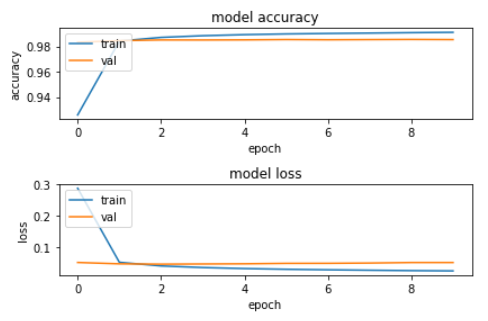
\includegraphics[width=\linewidth]{englishTraining.PNG}}
\caption{English Training}
\label{fig5}
\end{figure}

% CREATES IMAGE FIGURE
\begin{figure}[htbp]
\centerline{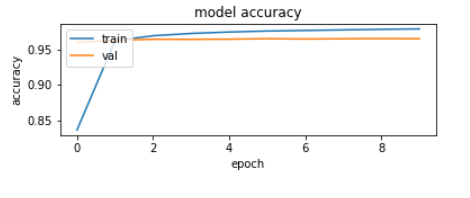
\includegraphics[width=\linewidth]{englishmasked.PNG}}
\caption{Masked Training for English}
\label{fig6}
\end{figure}

\subsubsection{Latin Model}
The Latin model reached an accuracy of 98.01\% and a masked accuracy of 93.62\% after testing with 8,162 sentences. 

% CREATES IMAGE FIGURE
\begin{figure}[htbp]
\centerline{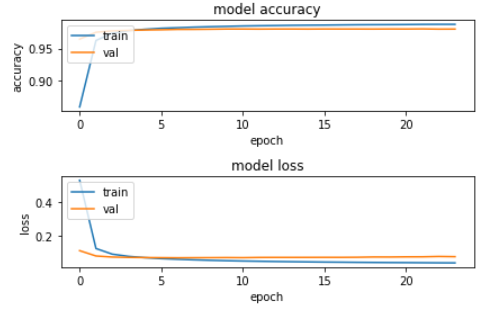
\includegraphics[width=\linewidth]{latinTraining.PNG}}
\caption{Latin Training}
\label{fig7}
\end{figure}

% CREATES IMAGE FIGURE
\begin{figure}[htbp]
\centerline{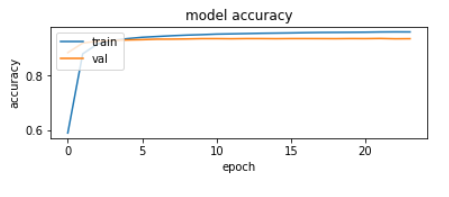
\includegraphics[width=\linewidth]{latinmasked.PNG}}
\caption{Masked Training for Latin}
\label{fig8}
\end{figure}

\subsection{Qualitative}
When unique sentences were fed as input to the model, there were between zero and two words tagged incorrectly. It was found that the model had more verb/adjective confusion than verb/noun or noun/adjective confusion. For example in the sentences, “I do not approve of his conduct,” and “I will conduct the symphony,” the model correctly tagged the word “conduct” as a noun in the first sentence and a verb in the second sentence. On the other hand, in the sentence “The old, tired man was sitting,” the model incorrectly tagged the word “tired” as a verb when it should have been tagged as an adjective. This verb/adjective confusion is rated higher than any verb/noun or noun/adjective confusion due to the fact that these words tend to be visually similar and placed in the same sections of a sentence. To the model, “tired” looks like a verb in past-tense, and it follows a determiner and an adjective as a verb normally might. These patterns are qualitatively more difficult for the model to learn.

For testing, the network was fed a simple sentence and it was decided if the network needed more time/data to learn based on whether it could correctly decipher the parts-of-speech in the sentence. The success or failure of the project hinged on the test cases succeeding.
The following is an example of how the model predicts and tags the various parts-of-speech for a sentence in English:

% CREATES IMAGE FIGURE
\begin{figure}[htbp]
\centerline{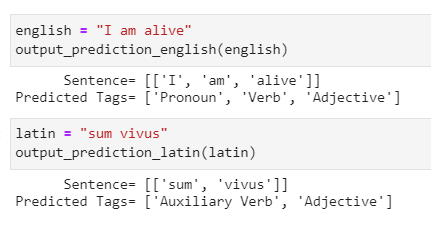
\includegraphics[width=\linewidth]{iamalive.PNG}}
\caption{Test Example}
\label{fig4}
\end{figure}  

\section{Discussion and Conclusion}
    The aim of the project was to create a part-of-speech tagger. For example, if the sentence “I am alive” was given as input to the tagger, the output would be: “Pronoun Verb Adjective”. The tagger was meant to be basic at first to allow for a better understanding of neural networks and natural language parsers. As the project evolved, the network was expanded to handle other languages, eventually moving to the classical language Latin. The success of this network will hopefully culminate into something that can assist with analysis of sentence structures and syntax. This application would be useful for linguists as well as those trying to learn a new language. Although this neural network began with English, it was extended to work with Latin and could be trained to perform with other languages given that an extensive and tagged dataset is available.
    
    Coding the ability to decipher a word’s part-of-speech based on syntax would be extremely difficult. This is why training a neural network to decipher a sentence's parts-of-speech was more desirable than having to write a case for every possible syntax/sentence structure. Given that every language has many grammar rules as well as exceptions to those rules, hard-coding this task would be impossible. For example, the network was able to differentiate between "conduct" in the earlier example sentences “I do not approve of his conduct” and “I will conduct the symphony”.
    
    The CNN worked remarkably well for this project. There were not many modifications made to the English part-of-speech tagging model to get it to perform well with Latin. Percent accuracy was found to be a little lower for the Latin model, but that is to be expected considering that the English model was trained using 61,371 sentences and the Latin model was trained using a smaller dataset of just 46,249 sentences. One of the limitations in extending this project to the classical language of Latin was the fact that there were more hand-tagged English sentence datasets for training, whereas it was difficult  to find as many hand-tagged Latin datasets. 
    
    The results of this project can be used by linguists and artificial intelligence scientists to assist in their research of natural language processing. While natural language processing in artificial intelligence has made great strides in recent years, it still has a long ways to go before it achieves human-like accuracy and ability. This project demonstrates that neural networks, specifically CNNs, have a future in natural language processing.


\bibliographystyle{IEEEtran}
\bibliography{References}

\end{document}
